% Results -- budget 1870 words (body text).
% Sources: docs/results_summary.md sections 5-11 (incl. 9.2d deep baselines, 10.1b outages and 10.2b forecasting on
% 30 datasets); docs/findings.md F01-F07, F16, F17, F21-F24, F30, F41-F47, F50, F51, F55-F59, F61-F63;
% results/catalogue_final/catalogue.csv (404 entries; rule-item confidence). Table rows generated from the result
% CSVs with half-up rounding (table5_detection.csv + deep_baselines/table_deep_baselines.csv, table6_attribution.csv,
% table8_forecasting.csv + forecast_all/forecast_summary.csv + dm_real.csv, transfer_tetouan/table9_detection.csv).
\section{Results}\label{sec:results}

\subsection{What the telemetry contains}\label{sec:res-telemetry}

The rule engine finds 327 items in the real data (126 dead, 155 fill, 33 clock and 13 transfer items), linked into 230 episodes. Straight-line fills, which the initial typology did not anticipate, are the most common fill mechanism: 85 fill items are pure straight lines, 54 pure holds and 16 mixed, and the first difference along a line is constant to about $10^{-14}$. Large events are compound episodes. In January 2023 (Fig.~\ref{fig:jan2023}) all 15 southern zones are filled at once, with holds in Laâyoune, Boujdour and one Foum El Oued zone and straight lines in the other six, and two days later all 15 zones are zero-filled for 13.7~h; the labels are A2, A2 and A1. In the episode of 31 March 2024 (Fig.~\ref{fig:mar2024}), held zones and zero-filled zones run side by side for 45.8~h: an acquisition state, not an electrical one.

No regional outage remains in the data. The regional-outage rule never fires, and all three multi-city dead events carry hold or straight-line evidence. The only regional-outage candidate, 16 July 2023, combines exact zeros in Boujdour and Foum El Oued with straight lines in every Laâyoune zone and is labelled an acquisition failure (A1, 0.93). The hypothesised restoration of grid events (Section~\ref{sec:typology}) is not supported either: 25 of the 117 southern dead runs (21\%) end in a straight line from the last zero to the first reading, so an apparent ramp is often an interpolation, and the learned evidence of the overshoot rule is almost nil ($\log(a/b) = 0.12$, against 1.8--4.8 for every other rule).

Clock errors follow the European, not the Moroccan, clock changes: the hour 02:00--02:50 is recorded twice on 30 October 2022 and 29 October 2023, and after the first date the daily profile is shifted by $\delta^* = -60$~min in all three cities.

Artefacts dominate the anomalous time. Counting every dead state as an outage gives 1,220.5 zone-hours in 117 runs; counting only the items typed as grid events gives 294.0 zone-hours in 79 runs, 4.15 times less. Zero fills (A1) alone account for 926.5 zone-hours.

\begin{figure}[tbp]
\centering
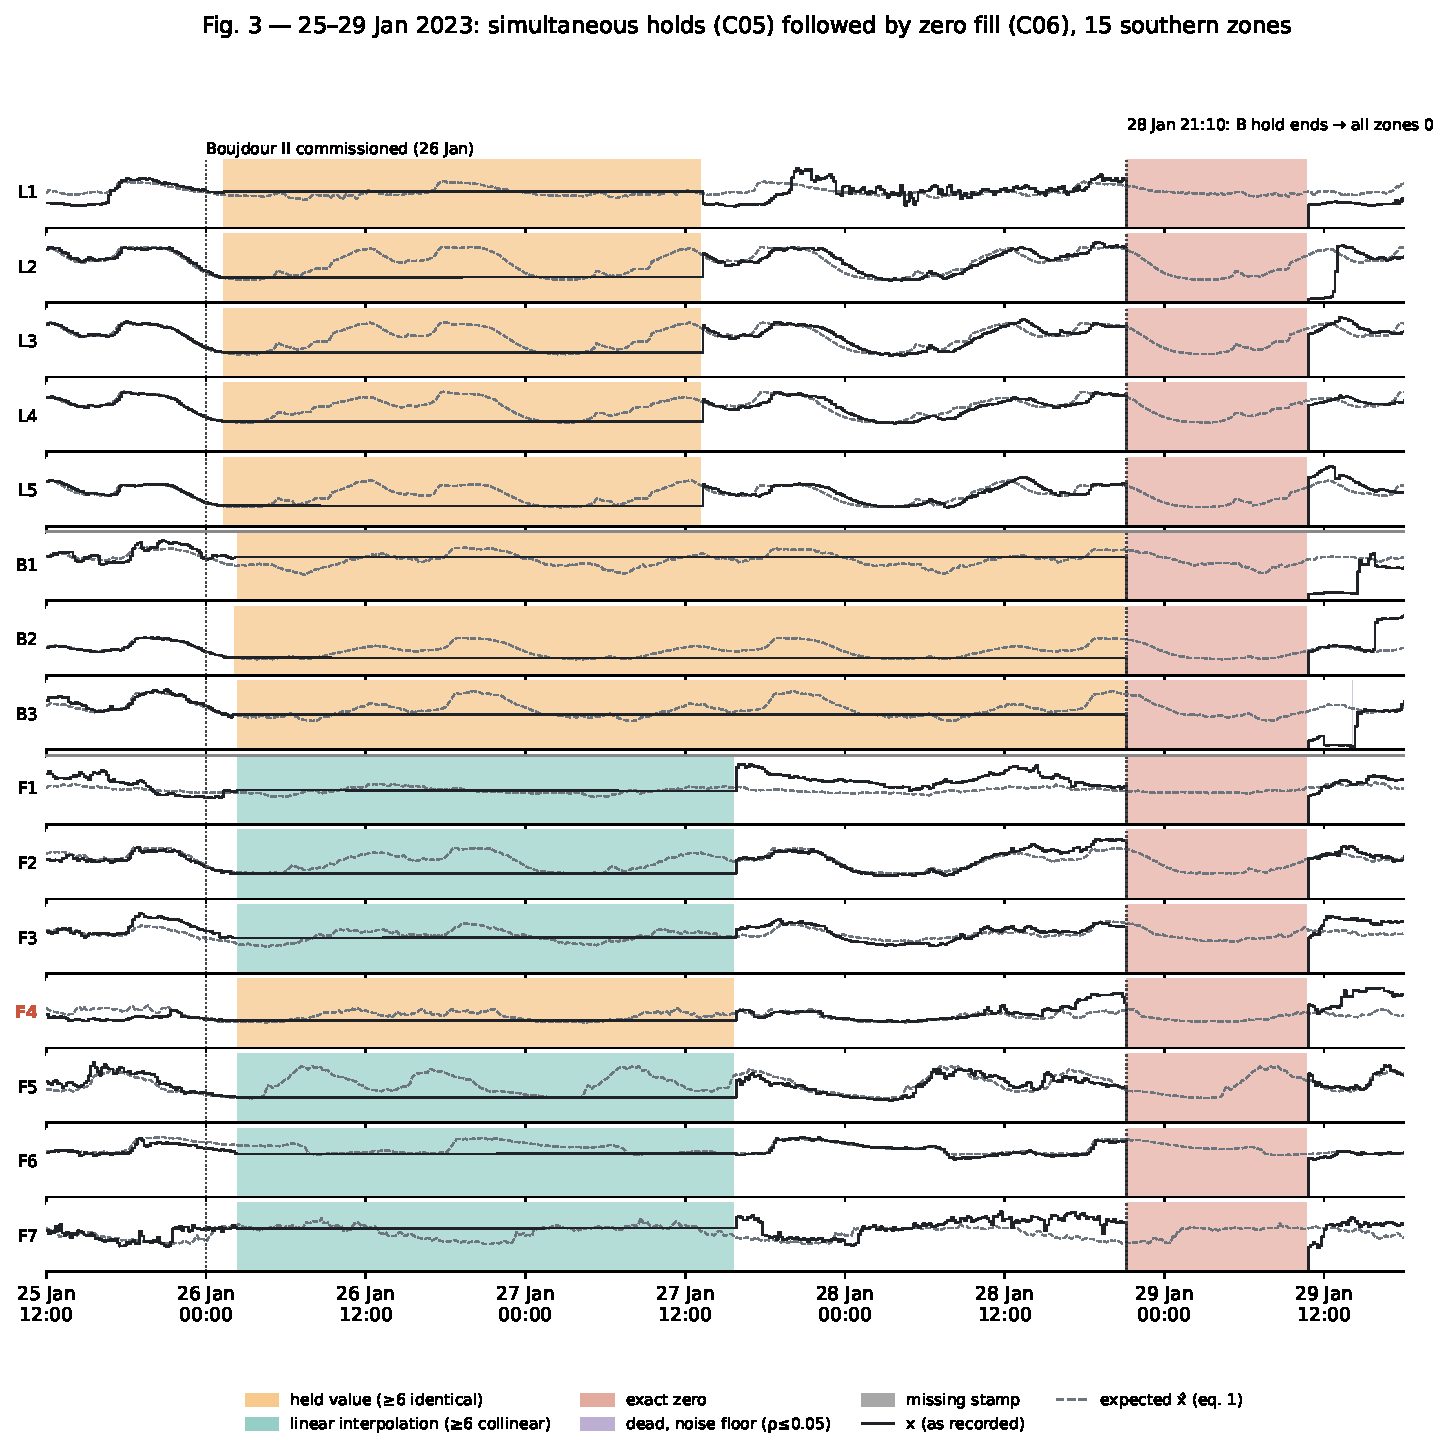
\includegraphics[width=\textwidth]{Figure_4}
\caption{The January 2023 acquisition episode (time stamps as recorded). Simultaneous holds (Laâyoune, Boujdour and F4) and straight-line fills (the other Foum El Oued zones) cover all 15 southern zones on 26--27 January; on 28 January all 15 zones are zero-filled for 13.7~h. Final labels A2, A2, A1.}
\label{fig:jan2023}
\end{figure}

\begin{figure}[tbp]
\centering
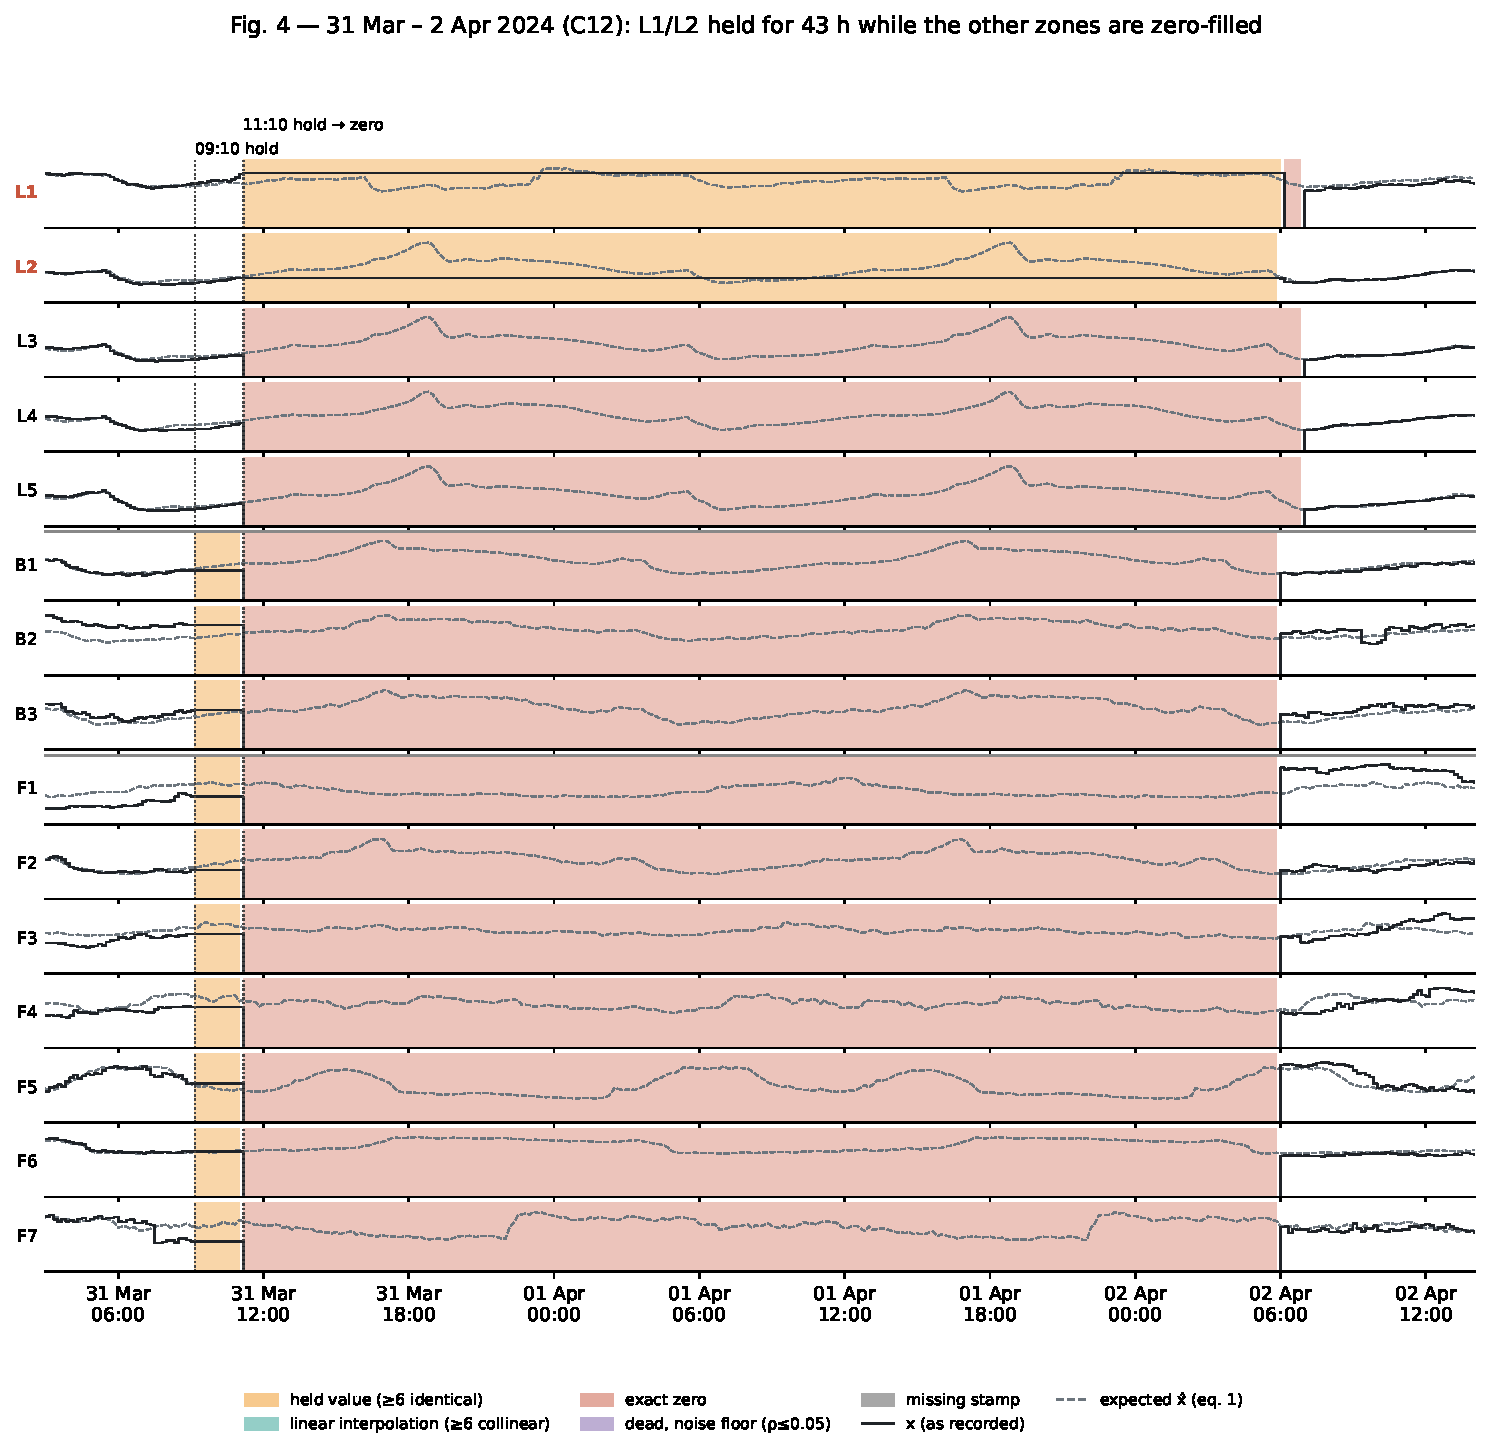
\includegraphics[width=\textwidth]{Figure_5}
\caption{The episode of 31 March -- 2 April 2024: Boujdour, Foum El Oued and L3--L5 are zero-filled while L1 and L2 are held. Final labels A2, A1, A2, G4; the last item, on L1, shows a limitation of the item-level label model (Section~\ref{sec:discussion}).}
\label{fig:mar2024}
\end{figure}

\subsection{Weak supervision on the real data}\label{sec:res-ws}

The constrained label model is stable where the standard one is not: its 20 restarts agree on every item, whereas restarts of the unconstrained Dawid--Skene model agree on as few as 62.7\% of the items (mean 83.2\%). On votes simulated from the fitted model, it recovers the true types with accuracy 0.922 and macro-F1 0.872 and is calibrated (ECE 0.033); the unconstrained model reaches 0.682, 0.493 and 0.276. Its labels agree with the rules' majority vote on 98.2\% of the items, but they come with probabilities: the mean confidence of the final rule-item labels is 0.937, and 13 items fall below 0.7.

The labels rest on the evidence one would expect. Dropping the straight-line rules changes 98.1\% of the fill labels and dropping the calendar rules 38.9\% of the dead labels, whereas dropping the simultaneity, restoration or single-zone rules changes none (supplementary material).

The released catalogue holds 404 entries: 327 rule items and 77 detector-only candidates (70 in the southern system, 7 in Marrakech). The rule items are labelled A3 98, G4 70, A2 57, G3 52, A4 14, A1 3, G2 1 and G5 1 (Table~\ref{tab:typology}), and 58 of the 70 southern candidates are untyped (N): partial drops, surges and short disturbances outside the typology.

\subsection{The residual hierarchy on the real data}\label{sec:res-hierarchy}

The hierarchy localises outages but not fills (Fig.~\ref{fig:hierarchy}). During the zero fills of January 2023, July 2023 and March 2024, the region part $g$ reaches robust $z$-scores of 218, 230 and 176, while a single-feeder outage moves only the zone part. All three multi-city dead items peak at the region level, and 92\% of the single-zone dead items at the zone level. Fills behave differently: a hold or a straight line drifts away from each zone's own expected path by a different amount, so the shared part stays small; only 17\% of the multi-city fills peak at the region level and 55\% of the city-wide fills at the city level. Fills are therefore found by their signatures, through the rules, rather than by the hierarchy, which makes the rules and the detector complementary.

\begin{figure}[tbp]
\centering
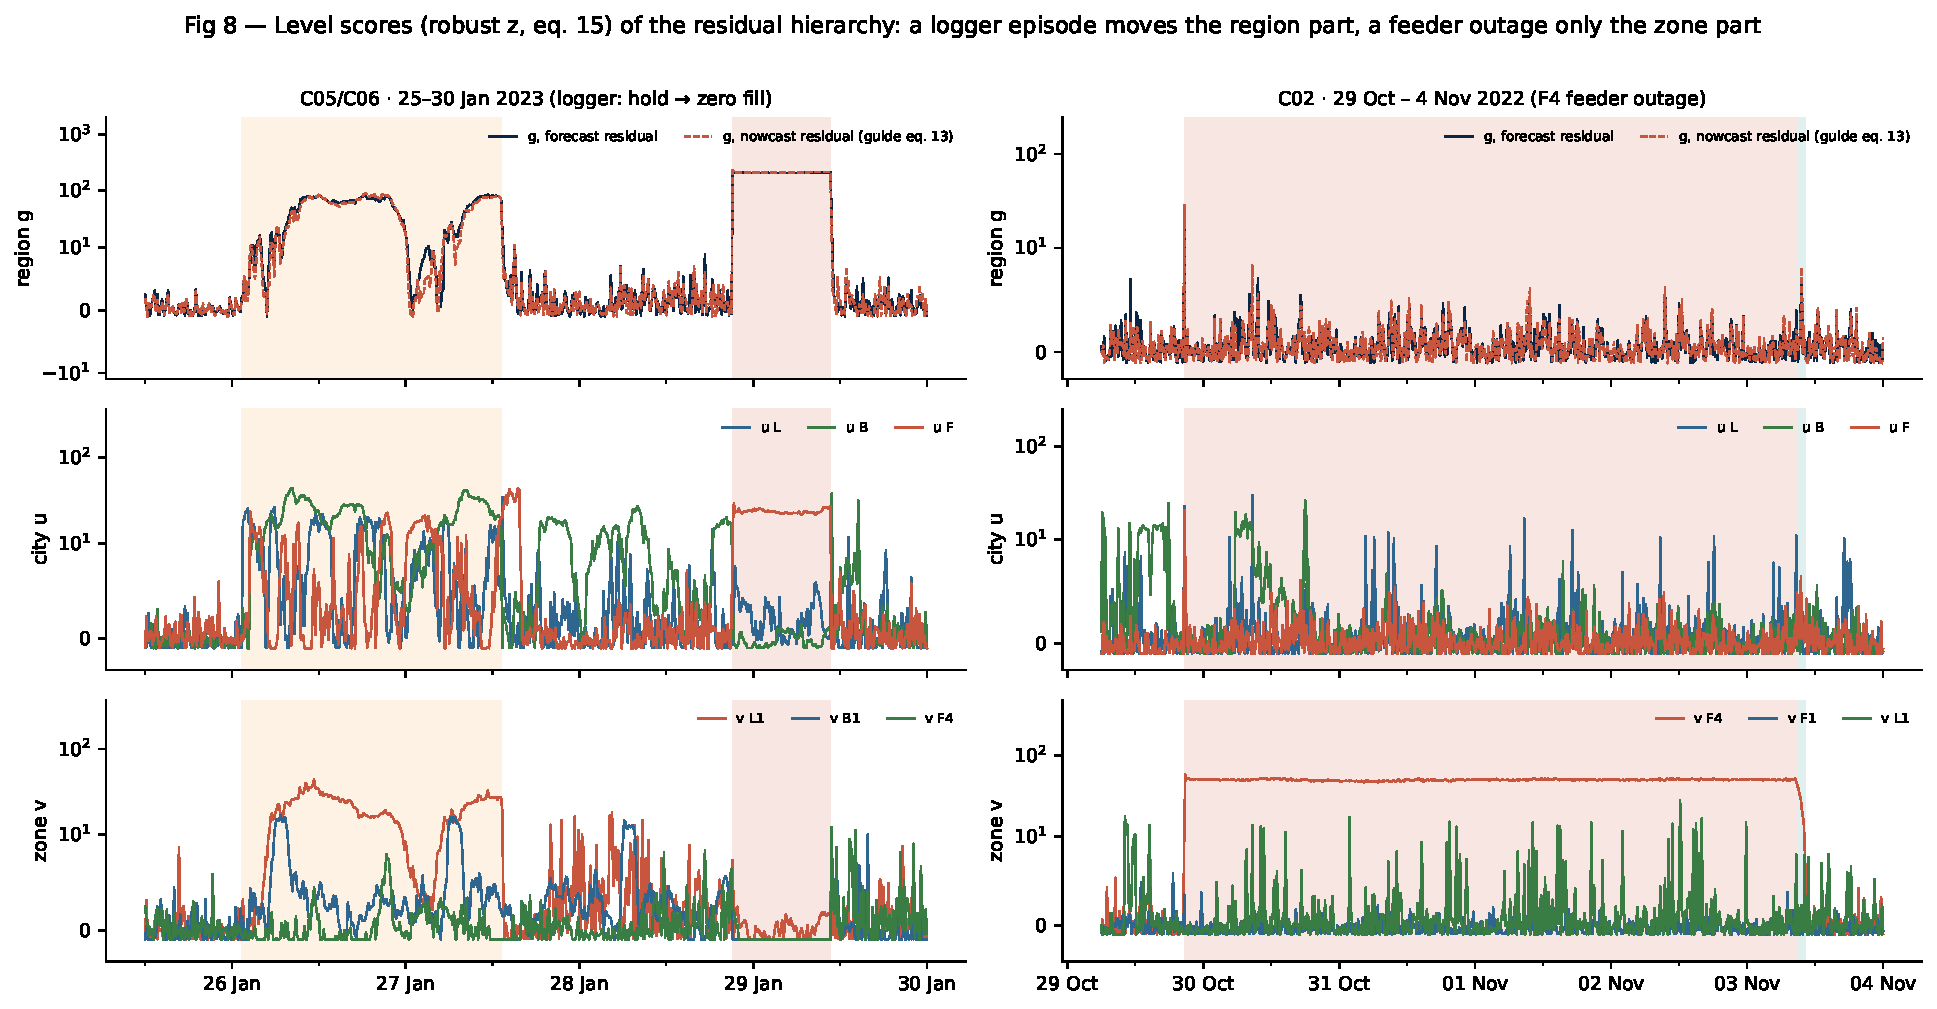
\includegraphics[width=\textwidth]{Figure_6}
\caption{Level scores (robust $z$-scores, Eq.~\eqref{eq:score}) of the residual hierarchy on the real data. During the January 2023 zero fill the region part $g$ reaches 218, while a feeder outage (F4, October 2022) moves only the zone part $v$. LightGBM residual; with the TCN-GAT residual, 73\% of the rule items peak at their structural level, against 71\%.}
\label{fig:hierarchy}
\end{figure}

\subsection{Detection on injected events}\label{sec:res-detection}

Fig.~\ref{fig:detection} and Table~\ref{tab:detection} compare the detectors. The rules alone reach event F1 0.86--0.90 at precision 1.00: they recall every injected type they were written for (city outages 0.90--0.94) and none of the untyped disturbances. The main detector is the best detector alone at 3\% and 7\% contamination (F1 0.813 and 0.854; Wilcoxon $p = 0.002$ against every other detector at 3\%, $p \le 0.020$ at 7\%); at 1\% (0.644) it is tied with the other residual detectors and STL ($p = 0.16$--$1.0$) and better than LOF and Isolation Forest. The deep baselines lose to the rules, to the main detector and to STL in every seed at every rate ($p = 0.002$): GDN reaches 0.37--0.71 and USAD 0.29--0.52. GDN finds 96--99\% of the multi-city zero gaps but fewer than 2\% of the single-zone fills, which are easy to forecast, and on clean data its forecasts are 7--14 times worse than the last value (supplementary material).

Adding the detector to the rules raises recall at every rate (0.82--0.84 against 0.76--0.81): it finds 5--30\% of the untyped city-wide shocks, 18--22\% of the partial drops and the city outages the rules miss. Its effect on F1 depends on how alarms are counted. If every alarm counts, the full method is worse than the rules at 1\% (0.721 against 0.863), equal at 3\% and better at 7\% (0.906 against 0.896, 10 of 10 seeds). If each method's own alarms on the uninjected series are excluded, as the rule states already are, it is better at every rate (0.90--0.91, $p = 0.002$). Under zone-strict matching it is worse at every rate: 25--75\% of the detector's extra alarms overlap an injected event in time but on other zones, because a zone left normal while its neighbours drop stands out at the city or region level.

The ablations (Fig.~\ref{fig:ablations}) locate the gain. Removing the learned graph leaves F1 equal or slightly higher ($+0.027$, $+0.004$ and $+0.003$): the graph adds interpretability, through the learned cross-city dependencies, but no detection skill. The tuned event formation contributes most ($-0.28$, $-0.14$ and $-0.02$ without it), followed by the multi-scale bands at low contamination ($-0.05$ and $-0.04$ at 1 and 3\%). A flat residual instead of the region--city--zone hierarchy does not lower F1 consistently: the hierarchy serves localisation, not detection. Smoothing costs timing: the median onset error is 140--168~min, against 60--70~min for STL.

\begin{figure}[tbp]
\centering
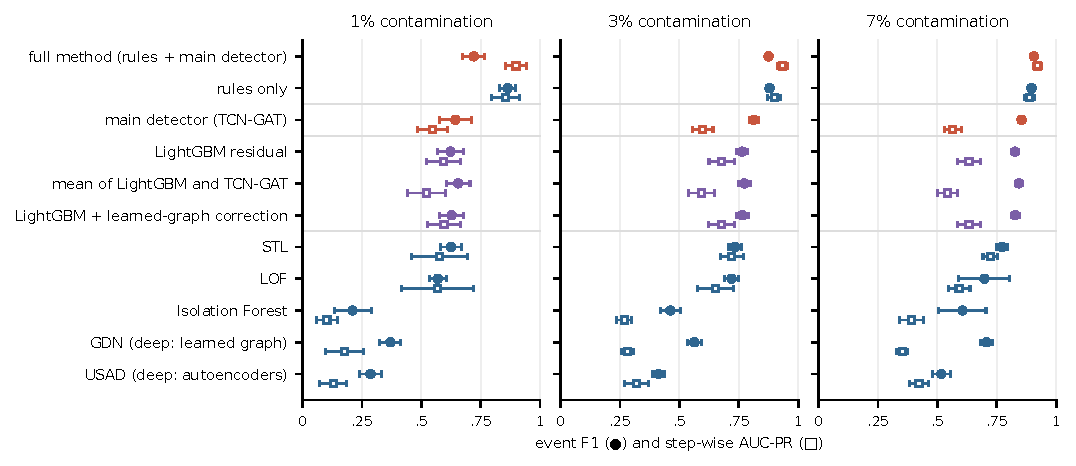
\includegraphics[width=\textwidth]{Figure_7}
\caption{Detection on injected events, test period: event F1 (circles, Eq.~\eqref{eq:eventf1}) and step-wise AUC-PR (squares), mean $\pm$ s.d. over 10 seeds at 1, 3 and 7\% contamination. Red: the full method and the main detector; purple: other predictors in the same residual detector; blue: the rules and the baselines, classical and deep. The ablations of the main detector are in Fig.~\ref{fig:ablations}.}
\label{fig:detection}
\end{figure}

\begin{table}[tbp]
\centering
\caption{Detection on injected events: the views that Fig.~\ref{fig:detection} does not show. Test period, mean over 10 seeds at 1 / 3 / 7\% contamination. Own background excluded: each method's own alarms on the uninjected series are not scored. Zone-strict: a match also requires a shared zone. Real-data alarms: alarms of the detector alone on the uninjected southern series (full method, i.e. the rules and the main detector: its detector-only candidates). LightGBM residual: the main detector with a LightGBM predictor and its own event formation.}
\label{tab:detection}
\scriptsize
\setlength{\tabcolsep}{3.5pt}
\begin{tabular}{@{}l c c c c r@{}}
\toprule
& & & F1, own background & Zone-strict & Real-data \\
Method & Precision & Recall & excluded & F1 & alarms \\
\midrule
Full method & 0.65/0.92/0.98 & 0.82/0.83/0.84 & 0.90/0.91/0.91 & 0.63/0.78/0.81 & 70 \\
Rules alone & 1.00/1.00/1.00 & 0.76/0.79/0.81 & 0.86/0.88/0.90 & 0.86/0.87/0.88 & -- \\
\midrule
Main detector & 0.58/0.89/0.98 & 0.73/0.75/0.76 & 0.82/0.84/0.85 & 0.62/0.78/0.81 & 191 \\
LightGBM residual & 0.57/0.82/0.96 & 0.69/0.72/0.73 & 0.79/0.82/0.83 & 0.61/0.74/0.77 & 152 \\
\midrule
STL & 0.64/0.87/0.97 & 0.62/0.64/0.64 & 0.74/0.76/0.76 & 0.61/0.71/0.71 & 178 \\
LOF & 0.51/0.77/0.91 & 0.66/0.68/0.57 & 0.71/0.76/0.70 & 0.55/0.69/0.64 & 263 \\
Isolation Forest & 0.14/0.37/0.65 & 0.48/0.63/0.57 & 0.39/0.63/0.65 & 0.17/0.42/0.53 & 457 \\
GDN & 0.27/0.52/0.78 & 0.60/0.62/0.65 & 0.68/0.70/0.74 & 0.29/0.46/0.57 & 366 \\
USAD & 0.23/0.49/0.76 & 0.38/0.36/0.39 & 0.43/0.45/0.48 & 0.23/0.35/0.41 & 243 \\
\bottomrule
\end{tabular}
\end{table}

\begin{figure}[tbp]
\centering
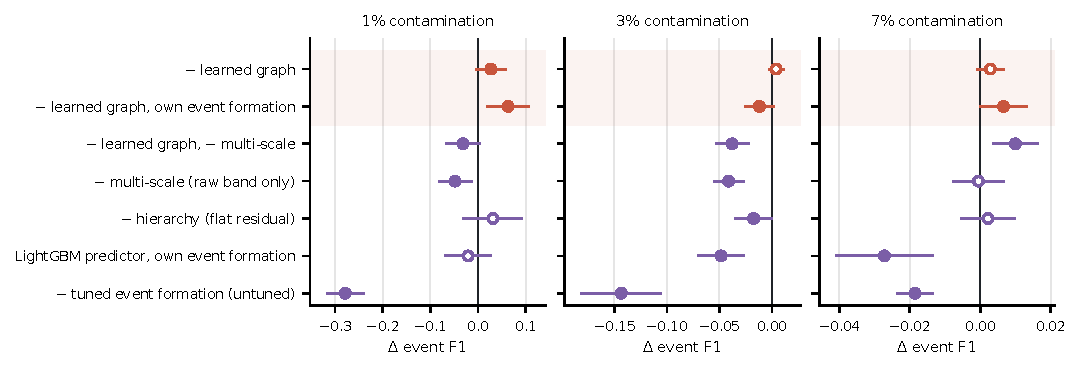
\includegraphics[width=\textwidth]{Figure_8}
\caption{Ablations of the main detector: change in event F1 relative to the main detector (mean $\pm$ s.d. of the per-seed differences; filled markers: Wilcoxon $p < 0.05$). The learned-graph ablation (shaded) leaves F1 equal or slightly higher; the multi-scale bands and the tuned event formation carry the gain.}
\label{fig:ablations}
\end{figure}

\subsection{Attribution}\label{sec:res-attribution}

On the injected events that the full method detects, every labeller reaches macro-F1 0.85--0.94 (Table~\ref{tab:attribution}). The label model does not beat the rules' majority vote on these signatures (0.900--0.934 against 0.913--0.940), the fusion matches both (0.906--0.944), and the end model alone is weaker at low contamination. What weak supervision adds is a calibrated probability for each label: the expected calibration error of the label model and of the fusion stays between 0.07 and 0.10 without recalibration (Fig.~\ref{fig:attribution}b). End to end, 0.90--0.95 of the typed injected events are both detected and correctly typed.

One confusion dominates (Fig.~\ref{fig:attribution}a): at 3\%, 44 of 160 zero-fill gaps (A1) are labelled regional outages (G1). The injected gaps drop to exactly zero in several cities at once, the simultaneity rules vote for a regional event, and nothing else separates the two; the real multi-city gaps also carry fill evidence, which the injector does not copy. Without the simultaneity rules the label model's A1 accuracy would rise from 0.70 to 0.83 and its macro-F1 from 0.914 to 0.941; we report this but do not adopt it, because it was observed on the test seeds. The other classes reach F1 0.86--0.99; feeder outages are sometimes taken for planned work (15 of 123).

\begin{table}[tbp]
\centering
\caption{Attribution of the injected events detected by the full method (test period; macro-F1 over the seven typed classes, mean $\pm$ s.d. over 10 seeds, and the mean expected calibration error, Eq.~\eqref{eq:ece}). Majority vote gives no probabilities.}
\label{tab:attribution}
\footnotesize
\setlength{\tabcolsep}{2.5pt}
\begin{tabular}{@{}l ccc ccc@{}}
\toprule
& \multicolumn{3}{c}{Macro-F1} & \multicolumn{3}{c}{ECE} \\
\cmidrule(lr){2-4}\cmidrule(l){5-7}
Labeller & 1\% & 3\% & 7\% & 1\% & 3\% & 7\% \\
\midrule
Majority vote & 0.940 $\pm$ 0.054 & 0.921 $\pm$ 0.029 & 0.913 $\pm$ 0.015 & -- & -- & -- \\
Label model $q$ & 0.934 $\pm$ 0.055 & 0.914 $\pm$ 0.029 & 0.900 $\pm$ 0.017 & 0.068 & 0.089 & 0.099 \\
End model $f$ & 0.845 $\pm$ 0.071 & 0.874 $\pm$ 0.025 & 0.902 $\pm$ 0.018 & 0.107 & 0.078 & 0.061 \\
Fusion $p$ & 0.944 $\pm$ 0.037 & 0.919 $\pm$ 0.023 & 0.906 $\pm$ 0.019 & 0.074 & 0.090 & 0.100 \\
\bottomrule
\end{tabular}
\end{table}

\begin{figure}[tbp]
\centering
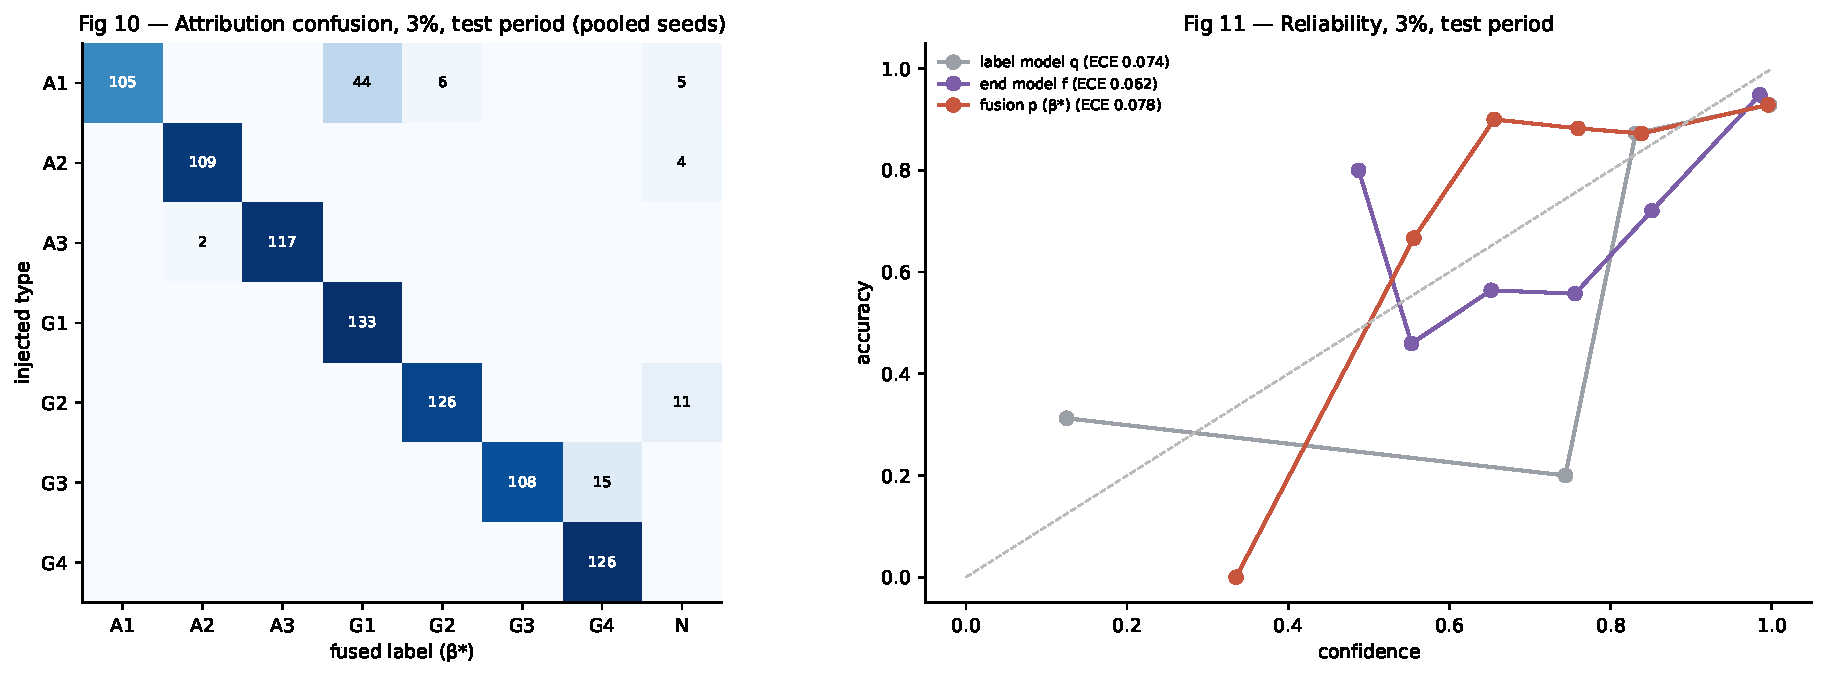
\includegraphics[width=\textwidth]{Figure_9}
\caption{Attribution on injected events (3\%, test period, seeds pooled): (a) confusion of the injected type and the fused label; (b) reliability of the label model $q$, the end model $f$ and the fusion $p$.}
\label{fig:attribution}
\end{figure}

\subsection{Outage statistics and forecasting}\label{sec:res-downstream}

On the injected data, where the truth is known, naive counting overstates outage zone-hours $1.88 \pm 0.32$ times and typed counting $1.26 \pm 0.24$ times (Fig.~\ref{fig:downstream}c). Typed counting is closer to the truth in all 30 datasets ($p = 1.9 \times 10^{-9}$) and recovers 99.8\% of the true outage zone-steps, and 99.98\% of its remaining excess lies inside injected zero-fill gaps: it is the A1-to-G1 confusion of Section~\ref{sec:res-attribution}, and nothing else. Interpolation (S1) erases outages from the record altogether. On the real data, the two counts differ 4.15-fold (Section~\ref{sec:res-telemetry}).

Type-aware cleaning also gives the most accurate forecasts when the forecaster reads the event indicator (Table~\ref{tab:downstream}, Fig.~\ref{fig:downstream}a--b). On the real data, the LightGBM day-ahead MASE after an anomaly falls from 1.501 (raw) and 1.233 (interpolated) to 1.061, 14\% below interpolation; the gain is significant at 1~h (DM $p < 0.001$) but not day-ahead ($p = 0.22$), because a few multi-zone events carry it. On the 30 injected datasets, S2 gives the lowest LightGBM error in 28--30 of them (Wilcoxon $p \le 5 \times 10^{-6}$) and comes within 0.006 MASE of the oracle S3. Over all test steps the effect is small, about 1\% against interpolation on the real data, because anomalies are rare. With the model-free reference the order changes: persistence and seasonal naive copy a kept outage into the next hour or day, so interpolation forecasts better (S1 beats S2 in all 30 datasets at 1~h), at the price of erasing the outages from the statistics.

\begin{table}[tbp]
\centering
\caption{Forecast error (MASE, Eq.~\eqref{eq:mase}) by cleaning strategy, test period 1 January -- 24 May 2024. After: steps within two days after an anomalous state in the zone; all: every scored step. Real data: S0 / S1 / S2 and the Diebold--Mariano $p$ of S1 against S2. Injected: S0 / S1 / S2 / S3, mean over the 30 test datasets, and the number of datasets in which S2 beats S1 with the Wilcoxon $p$ (S1 is better when the number is below 15).}
\label{tab:downstream}
\scriptsize
\setlength{\tabcolsep}{4pt}
\begin{tabular}{@{}l l l c c c c@{}}
\toprule
& & & \multicolumn{2}{c}{Real data} & \multicolumn{2}{c}{Injected data (30 datasets)} \\
\cmidrule(lr){4-5}\cmidrule(l){6-7}
Forecaster & Horizon & Steps & S0 / S1 / S2 & DM $p$ & S0 / S1 / S2 / S3 & S2 better (p) \\
\midrule
LightGBM & 1 h & after & 0.656/0.661/0.613 & $<$0.001 & 0.696/0.636/0.625/0.619 & 29 (4e-6) \\
LightGBM & 1 h & all & 0.654/0.657/0.654 & 0.019 & 0.653/0.625/0.625/0.620 & 28 (4e-6) \\
LightGBM & 1 day & after & 1.501/1.233/1.061 & 0.22 & 1.295/1.140/1.058/1.052 & 29 (5e-7) \\
LightGBM & 1 day & all & 1.140/1.115/1.102 & 0.25 & 1.174/1.076/1.052/1.051 & 29 (3e-6) \\
\midrule
Naive & 1 h & after & 1.081/1.059/1.052 & 0.44 & 0.995/0.920/0.939/0.923 & 0 (2e-9) \\
Naive & 1 day & after & 2.220/1.553/1.278 & 0.16 & 2.036/1.377/1.499/1.448 & 10 (6e-4) \\
\bottomrule
\end{tabular}
\end{table}

\begin{figure}[tbp]
\centering
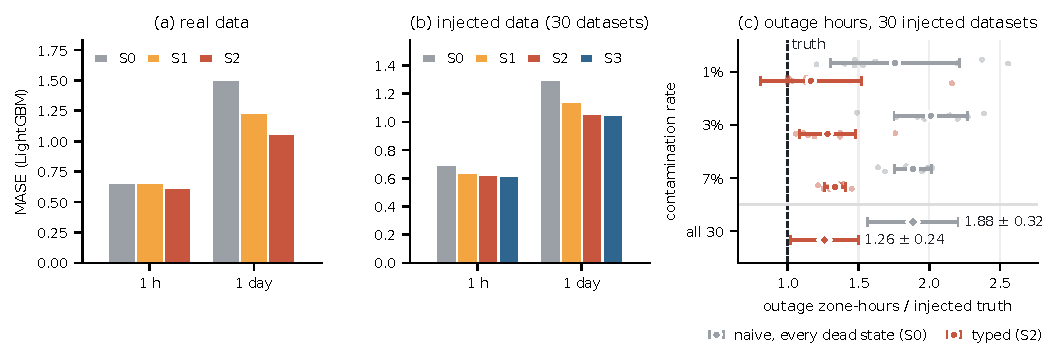
\includegraphics[width=\textwidth]{Figure_10}
\caption{Downstream test. LightGBM forecast error (MASE) by cleaning strategy on test steps within two days after an anomaly, (a) real data and (b) injected data (mean of 30 datasets); test period 1 January -- 24 May 2024. (c) Outage zone-hours relative to the injected truth under naive (S0) and typed (S2) counting on the 30 injected datasets (points: seeds; markers: mean $\pm$ s.d.). Interpolation (S1) reports no outage.}
\label{fig:downstream}
\end{figure}

\subsection{Transfer to Tetouan}\label{sec:res-transfer}

Tetouan tests the frozen method on another city and year (Fig.~\ref{fig:transferprotocol}). On the real 2017 series the rules raise no dead or fill item, and the four clock-change dates they examine are all labelled normal; the main detector raises 7 alarms in the year, 0.20 per zone-month, against 72 for Isolation Forest. On the injected datasets the full method reaches event F1 0.945, 0.919 and 0.890 at 1, 3 and 7\% contamination, at precision 0.98--1.00 (Table~\ref{tab:tetouan}, Fig.~\ref{fig:tetouan}a), and beats the rules alone (0.856--0.861) in every seed at every rate ($p = 0.002$). The main detector alone is the best detector at 1\% (0.857). At 3\% LightGBM and STL overtake it ($p = 0.002$ and 0.004), and at 7\% LightGBM and Isolation Forest ($p = 0.006$ and 0.002): on one year of three zones, the neural predictor forecasts four times worse than LightGBM (MAE 0.045 against 0.011).

Attribution transfers except for one class (Fig.~\ref{fig:tetouan}b). The frozen label model reaches macro-F1 0.77--0.79, and 0.95--0.98 without A1: 348 of 417 injected zero-fill gaps are read as city outages, with confidence above 0.98. In Morocco, a gap is told from an outage by its zeros in several cities at once; in a single city this evidence cannot exist.

\begin{figure}[tbp]
\centering
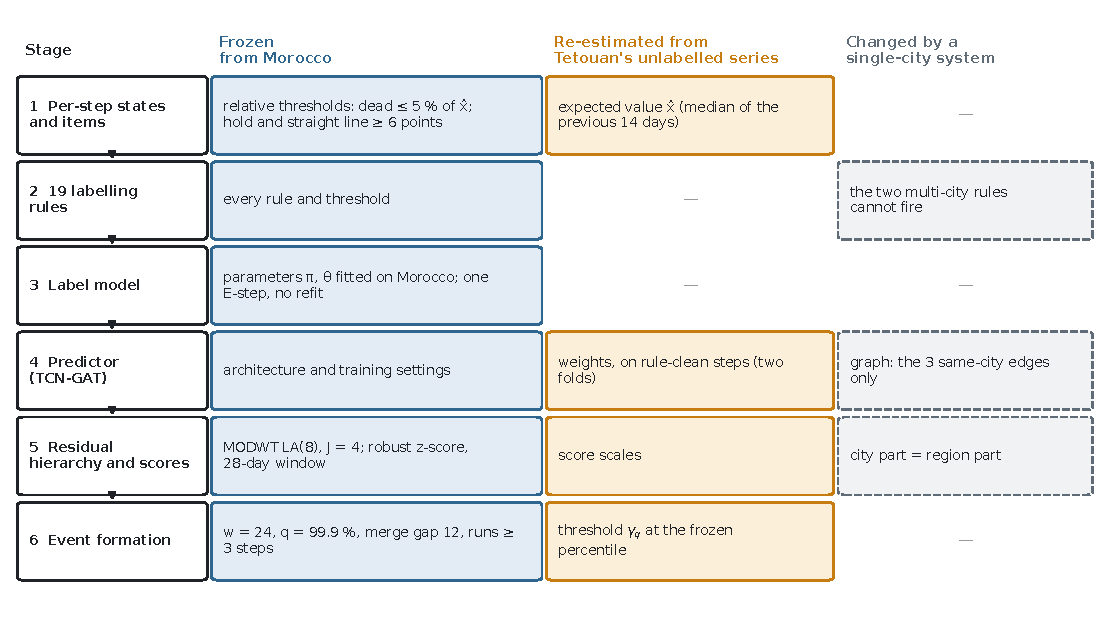
\includegraphics[width=\textwidth]{Figure_11}
\caption{Transfer protocol: what is frozen from the Moroccan system, what is re-estimated from Tetouan's unlabelled series, and what a single-city system changes.}
\label{fig:transferprotocol}
\end{figure}

\begin{table}[tbp]
\centering
\caption{Transfer to Tetouan without re-tuning (event F1 in Fig.~\ref{fig:tetouan}a). Injected data: mean over 10 seeds at 1 / 3 / 7\% contamination. Full method: the rules and the main detector. No graph: the main detector without the learned graph (same event formation). Real alarms: items or alarms raised on the real 2017 series (clock items labelled N excluded).}
\label{tab:tetouan}
\scriptsize
\setlength{\tabcolsep}{4pt}
\begin{tabular}{@{}l c c c r@{}}
\toprule
Method & Precision & Recall & AUC-PR & Real alarms \\
\midrule
Full method & 0.98 / 1.00 / 1.00 & 0.91 / 0.85 / 0.80 & 0.95 / 0.95 / 0.95 & 7 \\
Rules alone & 1.00 / 1.00 / 1.00 & 0.75 / 0.76 / 0.75 & 0.88 / 0.89 / 0.88 & 0 \\
\midrule
Main detector & 0.98 / 1.00 / 1.00 & 0.76 / 0.66 / 0.57 & 0.75 / 0.66 / 0.69 & 7 \\
Main detector, no graph & 0.99 / 1.00 / 1.00 & 0.72 / 0.65 / 0.55 & 0.52 / 0.57 / 0.61 & 9 \\
LightGBM residual & 0.75 / 0.98 / 1.00 & 0.79 / 0.78 / 0.62 & 0.84 / 0.82 / 0.83 & 15 \\
\midrule
STL & 0.77 / 0.97 / 1.00 & 0.72 / 0.72 / 0.59 & 0.80 / 0.78 / 0.81 & 13 \\
Isolation Forest & 0.35 / 0.61 / 0.90 & 0.81 / 0.81 / 0.73 & 0.42 / 0.54 / 0.66 & 72 \\
LOF & 0.76 / 0.90 / 0.70 & 0.73 / 0.62 / 0.12 & 0.66 / 0.59 / 0.29 & 11 \\
\bottomrule
\end{tabular}
\end{table}

\begin{figure}[tbp]
\centering
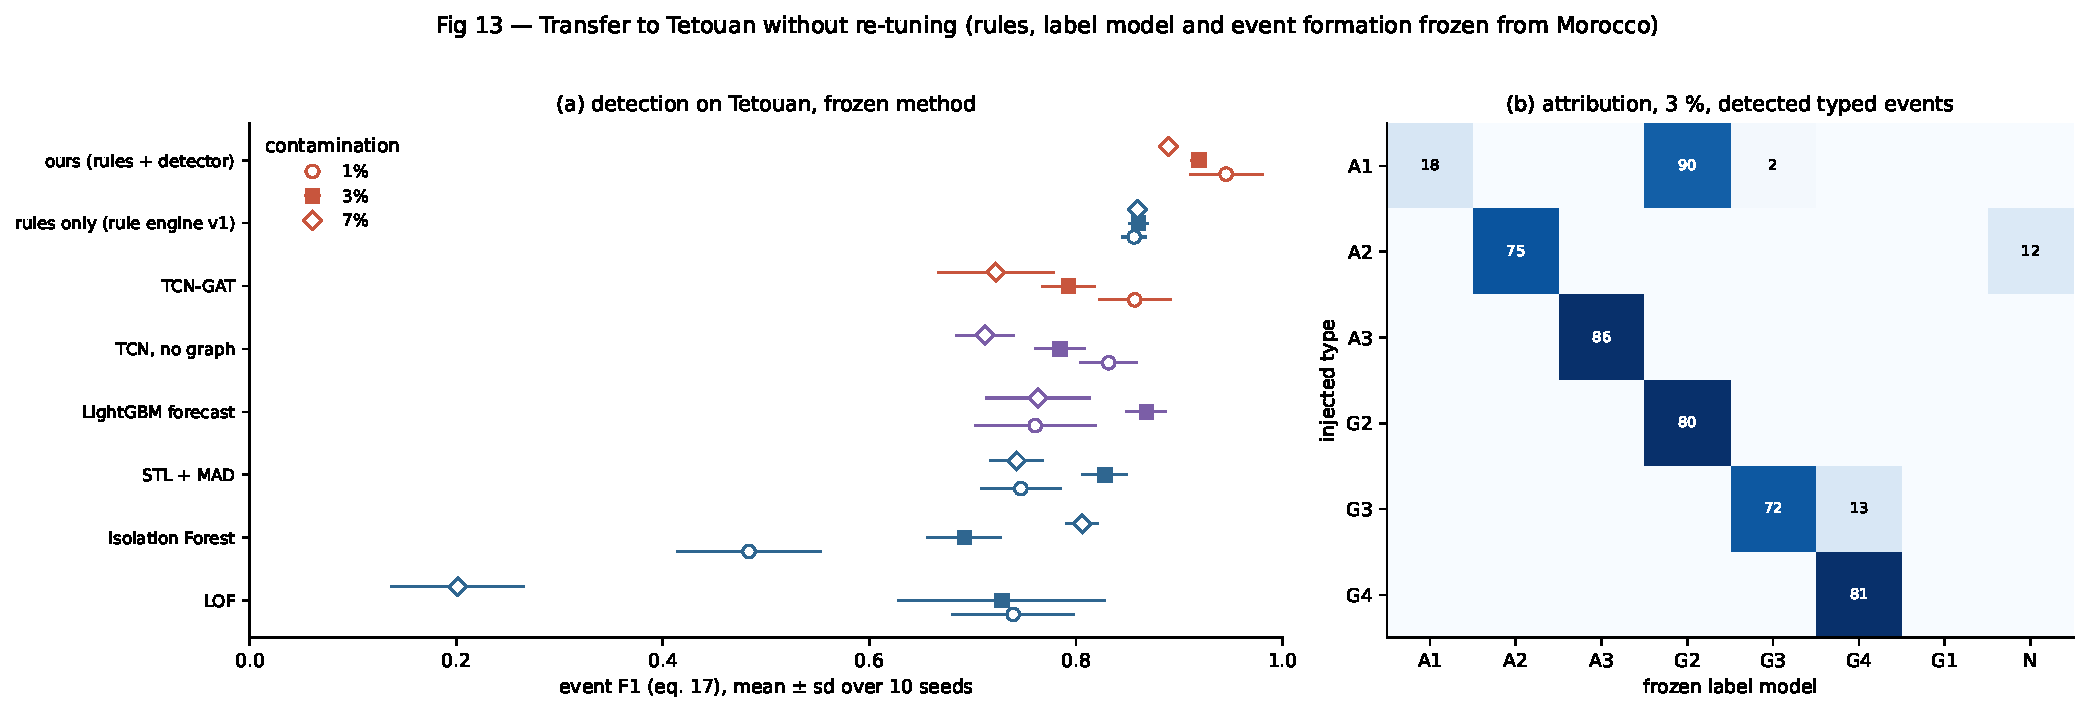
\includegraphics[width=\textwidth]{Figure_12}
\caption{Transfer to Tetouan without re-tuning: (a) event F1 of every method at 1, 3 and 7\% contamination; (b) confusion of the frozen label model at 3\%. City-wide zero gaps (A1) are read as city outages (G2).}
\label{fig:tetouan}
\end{figure}
